% =============================================================================
% DRAFTING NOTE (not part of the specification; delete before filing):
% This document is a drafting aid assembled from the technical content of
% paper.tex (ICASSP submission) for the purpose of preparing a U.S. provisional
% patent application. It is NOT legal advice and has NOT been reviewed by a
% registered patent attorney or agent. Before filing:
%   - Have a patent attorney/agent review scope, claim language, and
%     enablement/written-description sufficiency.
%   - Confirm inventorship (who actually conceived each claimed element) with
%     counsel -- inventorship is a legal determination, not an authorship list.
%   - Confirm whether "Institute of Brain and Mind" should be named as
%     applicant/assignee, and whether an assignment agreement is needed.
%   - A provisional application does not require formal claims, but including
%     illustrative claims (as done here) helps establish support for the
%     eventual non-provisional claims and is common practice.
%   - Check for any public disclosure (e.g., the ICASSP submission/preprint)
%     and file the provisional before or within any applicable grace period.
% =============================================================================

\documentclass[12pt]{article}
\usepackage[margin=1in]{geometry}
\usepackage{amsmath,amssymb}
\usepackage{graphicx}
\usepackage{tikz}
\usetikzlibrary{arrows.meta,positioning,fit,backgrounds,calc}
\usepackage{enumitem}
\usepackage[hidelinks]{hyperref}

\newcommand{\E}{\mathbb{E}}
\newcommand{\Var}{\operatorname{Var}}
\newcommand{\dhat}{\widehat{d}}

\newcounter{para}
\newcommand{\parnum}{\stepcounter{para}\noindent\textbf{[\thepara]}\quad}

\renewcommand{\baselinestretch}{1.5}

\begin{document}

\begin{center}
{\large\bfseries PROVISIONAL PATENT APPLICATION}\\[0.3em]
{\large\bfseries SYSTEM AND METHOD FOR REAL-TIME REMOVAL OF CARDIAC FIELD\\
ARTIFACT IN WEARABLE EAR-EEG USING HEARTBEAT-TIMING-REFERENCED\\
REPETITIVE DISTURBANCE REJECTION}
\end{center}

\vspace{1em}
\noindent\textbf{Inventors:} Wenlin Zhang, Sam Lin, Ye Yuan, Zheng Wang

\noindent\textbf{Affiliation:} Institute of Brain and Mind

\noindent\textbf{Applicant:} Institute of Brain and Mind

\vspace{1em}
\noindent\textbf{CROSS-REFERENCE TO RELATED APPLICATIONS}\\
Not applicable. This is a first-filed provisional application.

\vspace{0.5em}
\noindent\textbf{STATEMENT REGARDING FEDERALLY SPONSORED RESEARCH OR DEVELOPMENT}\\
Not applicable.

\vspace{0.5em}
\noindent\textbf{REFERENCE TO SEQUENCE LISTING, TABLE, OR COMPUTER PROGRAM LISTING}\\
Not applicable.

% =============================================================================
\section*{FIELD OF THE INVENTION}

\parnum This disclosure relates generally to wearable biosignal acquisition and processing, and more particularly to systems and methods for real-time cancellation of cardiac field artifact (CFA) in low-channel electroencephalography (EEG) signals acquired from ear-worn or head-worn devices, using heartbeat timing information rather than a full electrocardiogram (ECG) waveform as the reference.

% =============================================================================
\section*{BACKGROUND OF THE INVENTION}

\parnum Wearable EEG devices are increasingly designed for continuous, day-scale, low-channel operation in form factors such as in-ear or behind-the-ear earables, hearing-aid-like devices, and head-worn patches. These form factors place electrodes close to the neck and major vascular structures, making the recorded signal susceptible to contamination by the cardiac field artifact (CFA) -- the volume-conducted electrical potential generated by the heart -- which is distinct from the pulse-related ballistocardiographic artifact studied in EEG-fMRI contexts.

\parnum Existing approaches to removing cardiac-related artifact from EEG generally fall into two categories, each with practical limitations in the low-channel wearable regime:

\begin{enumerate}[label=(\alph*)]
\item \emph{Blind source separation methods} (e.g., independent component analysis, ICA) require a sufficient number of independent sensor channels to separate the cardiac source from neural sources. Low-channel earables (e.g., two to eight channels) typically do not provide enough spatial diversity for reliable separation.
\item \emph{Reference-driven adaptive cancellation methods} (e.g., least-mean-squares or recursive-least-squares adaptive noise cancellation referenced to a simultaneously recorded ECG or heartbeat waveform) require that the artifact waveform be predictable -- linearly or through a fixed nonlinearity -- from the reference waveform. In practice, near-ear electrode sites experience a different volume-conduction projection of the cardiac source than a chest-worn ECG lead, and the present inventors have measured near-zero waveform coherence between chest ECG and ear-EEG artifact even within R-peak-locked analysis windows (see Detailed Description). Under this condition, reference-driven waveform regression has little to no coherent structure to exploit, regardless of the adaptation algorithm used.
\end{enumerate}

\parnum A further practical constraint in the wearable ecosystem is that a heartbeat reference is frequently available not from a co-located, sample-synchronized ECG lead, but from a separate consumer device (e.g., a smartwatch providing ECG- or PPG-derived heartbeat timing). Cross-device timestamps are commonly available to modest precision, but the underlying analog waveform is not transferable in a sample-accurate, phase-coherent way because of unknown and variable inter-device latency and clock jitter. Prior reference-driven cancellation methods that depend on the reference \emph{waveform} are therefore poorly suited to this cross-device scenario, even though beat \emph{timing} may be perfectly usable.

\parnum There is accordingly a need for a CFA removal method suitable for low-channel wearable EEG that (i) does not depend on the number of EEG channels being large enough for blind source separation, (ii) does not require the cardiac artifact waveform to be predictable from an external reference waveform, and (iii) can be driven by heartbeat \emph{timing} alone, so that the reference may originate from a separate wearable device without requiring sample-accurate waveform synchronization between devices.

% =============================================================================
\section*{SUMMARY OF THE INVENTION}

\parnum The present invention addresses the above needs by treating the cardiac field artifact as a heartbeat-synchronous \emph{repetitive disturbance} in the sense of repetitive control and iterative learning control (ILC), and rejecting it by phase-indexed synchronous averaging/estimation keyed only to the timing of heartbeats (e.g., ECG R-peaks), rather than to the ECG waveform shape.

\parnum In one aspect, a method is provided for removing cardiac field artifact from a wearable EEG signal, comprising: (a) receiving a heartbeat timing reference identifying a sequence of heartbeat instants (e.g., R-peak times) from an ECG or PPG sensor, which may be co-located with the EEG sensor or located on a separate wearable device; (b) estimating, from the heartbeat timing reference, a cardiac phase value for each EEG sample, the phase being defined relative to elapsed time since the most recent heartbeat instant (a time-since-R offset) rather than a normalized 0-to-1 phase, so that systolic structure remains time-locked to the heartbeat while diastolic variation absorbs beat-to-beat interval changes; (c) constructing a phase-indexed template of the repetitive cardiac disturbance by averaging or recursively updating, at each phase offset, the EEG samples observed at that offset across multiple heartbeats; and (d) subtracting the phase-indexed template from the measured EEG signal to produce a cleaned EEG signal in which the heartbeat-locked artifact is attenuated while non-phase-locked neural activity is substantially preserved.

\parnum In a further aspect, the template construction of step (c) is performed in one of at least three operating modes selectable according to application latency requirements: (i) a \emph{non-causal} mode, suitable for offline processing, in which the template at each phase offset is the batch average of the EEG samples at that offset across all available heartbeats in a recording; (ii) a \emph{buffered causal} mode, suitable for near-real-time streaming, in which the template is updated recursively (e.g., by an exponentially-weighted iterative-learning-control update) using the most recently completed heartbeat, and the cleaned output for that completed heartbeat is produced with a latency of approximately one heartbeat interval; and (iii) a \emph{strict causal} mode, suitable for zero-added-latency real-time operation, in which the current, still-in-progress heartbeat's phase is estimated by a causal phase-locked-loop (PLL)-type tracker rather than waiting for the next detected heartbeat instant, allowing cancellation to be applied to the current sample at the cost of some suppression performance near the heartbeat instant due to phase-prediction jitter.

\parnum In a further aspect, the system includes an arrhythmia/quality supervisor that gates the template update of step (c): when an incoming heartbeat is detected as premature, missed, or otherwise unreliable (e.g., by RR-interval plausibility checking), the corresponding beat is excluded from the template update (and, optionally, cancellation is suspended for that beat), preventing corruption of the learned template by irregular beats.

\parnum In a further aspect, the system includes an amplitude limiter/safeguard that bounds the magnitude of the estimated disturbance template and/or its update rate relative to a running estimate of the local signal envelope, so that the canceller cannot remove more signal power than is consistent with a plausible cardiac artifact amplitude -- providing a safeguard against inadvertent attenuation of neural signal content in the event of phase-tracking error or template mis-estimation. In embodiments employing a reference-driven residual stage (e.g., a Hammerstein-type nonlinear reference expansion followed by a recursive-least-squares residual canceller) in addition to the repetitive-disturbance stage, an analogous leaky-adaptation safeguard bounds that stage's contribution.

\parnum In a further aspect, because the disclosed method depends only on heartbeat \emph{timing} and not on the heartbeat \emph{waveform}, the heartbeat timing reference of step (a) may be derived from a device physically separate from the EEG-acquisition device -- for example, a wrist-worn smartwatch providing ECG- or photoplethysmography (PPG)-derived beat timestamps communicated to the EEG device or a companion processor over a wireless link -- without requiring sample-accurate, phase-coherent synchronization of an analog or digitized waveform between the two devices. This is a specific, practical advantage over reference-waveform-driven adaptive cancellation architectures.

\parnum In a further aspect, template quality is assessed, without access to ground truth, by comparing the R-locked energy of the template computed on the true detected heartbeat instants against the R-locked energy computed on a phase-scrambled (e.g., circularly time-shifted) surrogate heartbeat instant sequence that preserves the beat-interval statistics but destroys absolute phase alignment; the ratio of these energies (expressed, e.g., in decibels) provides a quantitative, reference-free template signal-to-noise metric usable for quality control, channel selection, or adaptive gain scheduling in a deployed device.

\parnum In a further aspect, the same repetitive-disturbance-rejection architecture is applicable, with the heartbeat timing reference replaced by a timing reference derived from an inertial measurement unit (accelerometer and/or gyroscope), to the rejection of periodic or quasi-periodic motion artifact (e.g., gait-cycle-locked or repetitive-motion-locked artifact) in wearable EEG or other wearable biosignals, using the same phase-indexing, template-estimation, supervisor-gating, and amplitude-limiting mechanisms described above with the reference event stream replaced accordingly.

\parnum In a further aspect, a system embodying the above method is provided, comprising: an EEG sensor interface; a heartbeat-timing receiver (which may be an onboard ECG/PPG front end or a wireless receiver for beat timestamps from a separate wearable device); a phase estimator comprising a peak/beat detector and a phase-locked-loop-type tracker with an arrhythmia supervisor; a template estimator configured to operate in the non-causal, buffered-causal, or strict-causal modes described above; a subtractor that produces the cleaned EEG output; and, optionally, an amplitude-limited reference-driven residual-cancellation stage operative when the reference-to-artifact coherence is determined to be sufficient.

% =============================================================================
\section*{BRIEF DESCRIPTION OF THE DRAWINGS}

\parnum FIG.~1 is a block diagram of an exemplary embodiment of the disclosed system, showing the heartbeat-timing input, the phase estimator (beat detector, PI phase-locked loop, and arrhythmia supervisor), the phase-indexed repetitive-disturbance template estimator operating in non-causal, buffered-causal, or strict-causal mode, the amplitude limiter/safeguard, and the subtractor producing the cleaned EEG output.

\parnum FIG.~2 shows an example of non-causal repetitive-disturbance-rejection cancellation applied to a real ear-EEG recording segment, comprising a chest ECG channel with detected heartbeat instants (top) and the original versus cleaned ear-EEG signal (bottom), together with a phase-indexed template estimated from the full recording session.

\parnum FIG.~3 shows a coherence analysis on the same real recording, comparing (left) a single heartbeat-locked ECG waveform overlaid with the non-causal and buffered-causal EEG templates, and (right) the coherence between the windowed ECG beat and three heartbeat-locked EEG views (raw EEG beat, non-causal template, buffered template), illustrating that the artifact is timing-repeatable even though ECG-to-EEG waveform coherence remains low.

\parnum FIG.~4 shows results of a semi-synthetic simulation sweeping the coherence between a reference ECG-like signal and a synthetic cardiac artifact from high to near-zero at fixed artifact power, comparing signal-to-noise-ratio improvement achieved by a conventional reference-driven adaptive-noise-cancellation baseline against the disclosed non-causal and buffered repetitive-disturbance-rejection methods, showing that the disclosed methods remain effective across the full coherence range because they rely on heartbeat timing repeatability rather than reference waveform predictability.

\begin{figure}[h]
\centering
\resizebox{\linewidth}{!}{%
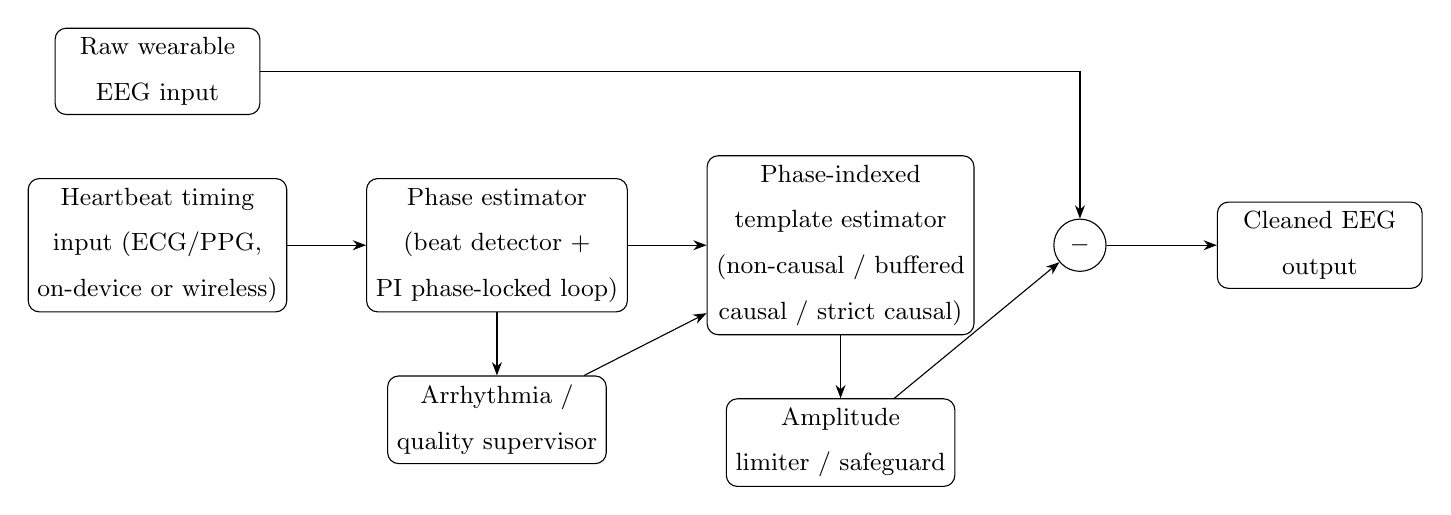
\begin{tikzpicture}[
  node distance=8mm and 10mm,
  block/.style={draw, rounded corners, align=center, minimum height=9mm, minimum width=26mm, font=\small},
  sum/.style={draw, circle, minimum size=6mm, font=\small},
  >=Stealth
]
\node[block] (ecg) {Heartbeat timing\\input (ECG/PPG,\\on-device or wireless)};
\node[block, right=of ecg] (phase) {Phase estimator\\(beat detector +\\PI phase-locked loop)};
\node[block, below=of phase] (sup) {Arrhythmia /\\quality supervisor};
\node[block, right=of phase] (tmpl) {Phase-indexed\\template estimator\\(non-causal / buffered\\causal / strict causal)};
\node[block, below=of tmpl] (lim) {Amplitude\\limiter / safeguard};
\node[sum, right=of tmpl] (sum1) {$-$};
\node[block, right=14mm of sum1] (out) {Cleaned EEG\\output};
\node[block, above=of ecg] (eeg) {Raw wearable\\EEG input};

\draw[->] (ecg) -- (phase);
\draw[->] (phase) -- (tmpl);
\draw[->] (phase) -- (sup);
\draw[->] (sup) -- (tmpl);
\draw[->] (tmpl) -- (lim);
\draw[->] (lim) -- (sum1);
\draw[->] (eeg) -| (sum1);
\draw[->] (sum1) -- (out);
\end{tikzpicture}%
}
\caption{FIG. 1 -- Block diagram of an exemplary embodiment of the disclosed system.}
\label{fig:patent_block_diagram}
\end{figure}

\begin{figure}[h]
\centering
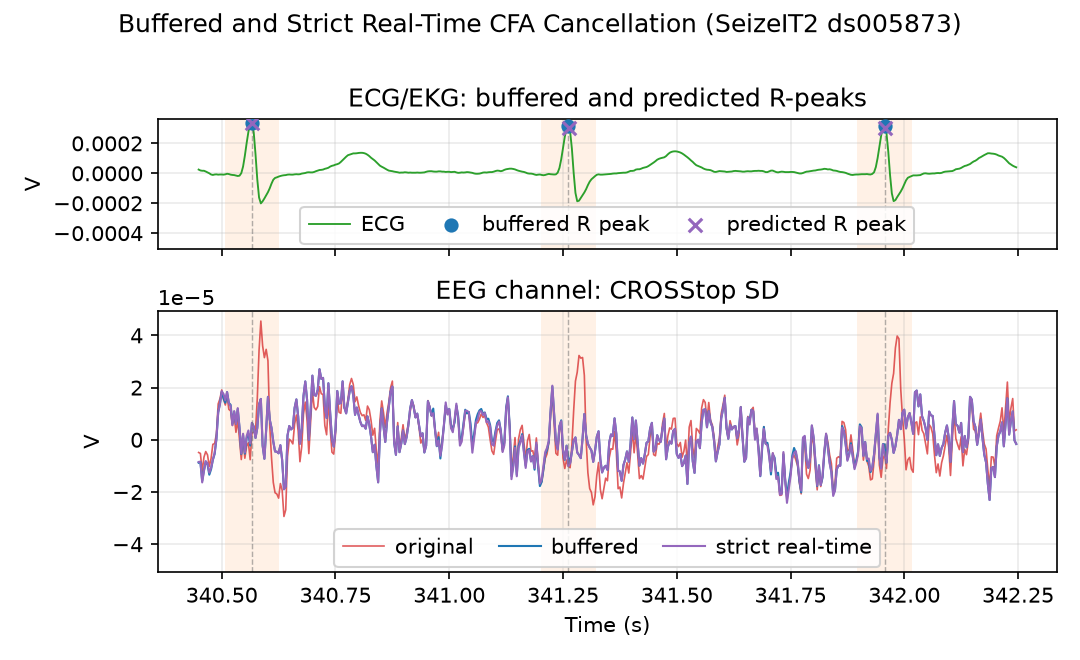
\includegraphics[width=0.85\linewidth]{fig_real/fig_noncausal_cleanup.png}
\caption{FIG. 2 -- Non-causal repetitive-disturbance-rejection cancellation on a real ear-EEG segment. Top: chest ECG with detected heartbeat instants. Bottom: original versus cleaned ear-EEG.}
\label{fig:patent_noncausal}
\end{figure}

\begin{figure}[h]
\centering
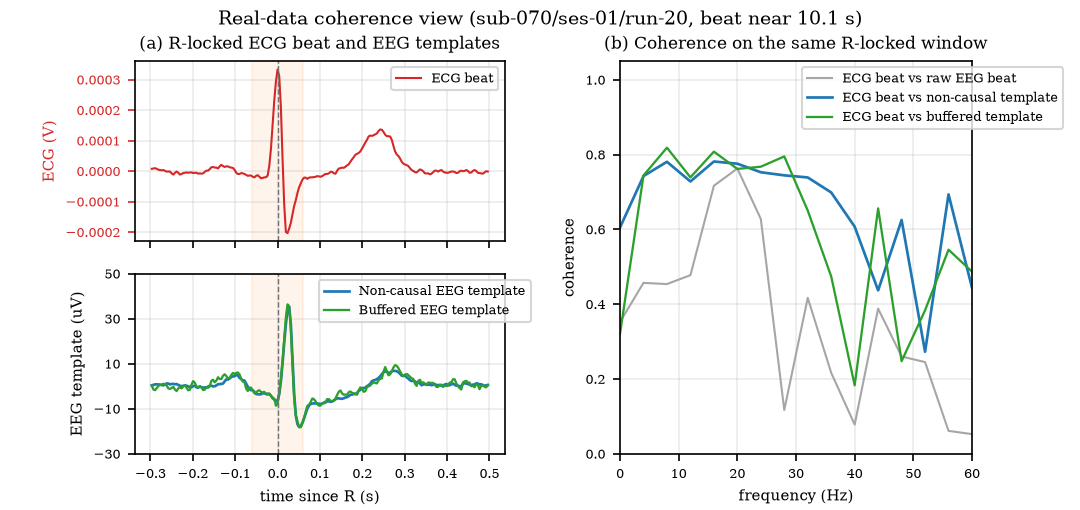
\includegraphics[width=0.85\linewidth]{fig_real/fig_real_coherence_combined.png}
\caption{FIG. 3 -- Coherence analysis on the same real recording. Left: heartbeat-locked ECG beat overlaid with the non-causal and buffered-causal EEG templates. Right: coherence between the windowed ECG beat and three heartbeat-locked EEG views.}
\label{fig:patent_coherence}
\end{figure}

\begin{figure}[h]
\centering
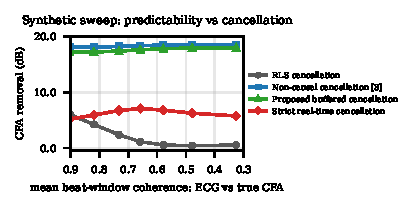
\includegraphics[width=0.85\linewidth]{fig3_synthetic_coherence_sweep.pdf}
\caption{FIG. 4 -- Semi-synthetic sweep of reference-to-artifact coherence versus cancellation performance, comparing a reference-driven adaptive baseline against the disclosed repetitive-disturbance-rejection methods.}
\label{fig:patent_synthetic}
\end{figure}

% =============================================================================
\section*{DETAILED DESCRIPTION OF THE INVENTION}

\subsection*{1. Signal model}

\parnum The measured wearable EEG signal $y(t)$ is modeled as
\begin{equation}
y(t) = s(t) + d_r(t) + n(t),
\label{eq:meas}
\end{equation}
where $s(t)$ is the neural signal of interest, $d_r(t)$ is the heartbeat-synchronous repetitive cardiac disturbance (the CFA), and $n(t)$ aggregates asynchronous interference and sensor noise. The disturbance period is set by the sequence of detected heartbeat instants $\{t_k\}$ (e.g., ECG R-peaks), with beat interval $T_k = t_{k+1}-t_k$.

\parnum It is assumed that: (i) the CFA is dominated by its repetitive component $d_r(t)$, with the R-peak-asynchronous disturbances and noise treated as zero-mean under heartbeat-synchronous averaging; (ii) the neural signal of interest $s(t)$ is not phase-locked to the heartbeat, so that its phase relative to the cardiac cycle is effectively uniform across beats, and it is therefore preserved (in expectation) by the phase-synchronous cancellation described below; and (iii) the beat period $T_k$ is accurately tracked and varies slowly (e.g., due to respiratory sinus arrhythmia), so that a shared phase grid may be used across beats.

\parnum The repetitive disturbance is represented as a function of a phase-index variable measured as elapsed samples $p$ since the associated heartbeat instant $t_k$ (a time-since-R offset), rather than as a normalized $0$-to-$1$ phase fraction of the beat interval. This choice keeps the systolic (R-spike-proximate) portion of the template time-locked in absolute time across beats -- since it is physiologically tied to the electrical depolarization event itself -- while allowing the diastolic (later) portion of the template window to absorb beat-to-beat variation in interval length. A person having ordinary skill in the art will appreciate that a normalized-phase indexing, or a hybrid indexing scheme, may be substituted without departing from the scope of the invention.

\subsection*{2. Non-causal (offline) template estimation and cancellation}

\parnum For a fixed phase offset $p$, a template value is estimated as the average, across $N_r$ heartbeats, of the EEG sampled at offset $p$ from each detected heartbeat instant $\hat t_k$:
\begin{equation}
\dhat_r(p) = \frac{1}{N_r}\sum_{k=1}^{N_r} y_k(p),
\qquad
y_k(p) \equiv y(\hat t_k + p/f_s),
\label{eq:est}
\end{equation}
where $f_s$ is the sampling rate. Because the repetitive component $d_r(p)$ is the same at every beat while the neural and noise components are not phase-locked, the sample average converges (as $N_r$ grows) to an estimate of the repetitive disturbance alone, with residual leakage variance scaling approximately as $V(p)/N_r$ for per-sample asynchronous variance $V(p)$. The cleaned signal is then formed as
\begin{equation}
\widehat{s}_k(p) \approx y_k(p) - \dhat_r(p).
\label{eq:ideal}
\end{equation}

\subsection*{3. Causal (streaming) template estimation and cancellation}

\parnum For streaming/real-time operation, the batch average of Eq.~\eqref{eq:est} is replaced by a recursive, exponentially-weighted update performed once per qualifying heartbeat at each phase offset $p$:
\begin{equation}
\hat{d}_r^{(k)}(p) = \hat{d}_r^{(k-1)}(p) + a\left[y_k(p) - \hat{d}_r^{(k-1)}(p)\right],
\label{eq:causal_ilc_update}
\end{equation}
where $a$ is a tunable learning gain trading off convergence speed against leakage of non-repetitive energy into the template, and the arrhythmia supervisor (Section 5, below) freezes this update on premature, missed, or otherwise unreliable beats.

\parnum In a \emph{buffered-causal} embodiment, the cleaned output for the just-completed beat $k-1$ is produced using the template as of that beat,
\begin{equation}
\widehat{s}_{k-1}(p) \approx y_{k-1}(p) - \hat{d}_r^{(k-1)}(p),
\end{equation}
introducing approximately one heartbeat interval of output latency in exchange for using the fully realized (detected) heartbeat instant for phase anchoring.

\parnum In a \emph{strict-causal} embodiment, cancellation is applied to the current sample before the current heartbeat's instant has been detected. Phase is instead anchored using a prediction from a causal phase-tracking loop (e.g., a proportional-integral phase-locked loop driven by the sequence of previously detected heartbeat instants and interval statistics), enabling zero added latency at the cost of reduced suppression performance in the immediate vicinity of the heartbeat instant, where phase-prediction jitter is largest.

\parnum Both the buffered-causal and strict-causal embodiments require only $O(1)$ arithmetic operations per input sample and $O(L_w)$ memory (where $L_w$ is the number of phase bins in the template window), making the method suitable for implementation on low-power embedded or wearable processors.

\subsection*{4. Phase/beat tracking}

\parnum A beat detector identifies candidate heartbeat instants from the timing reference signal (e.g., an ECG or PPG channel, or timestamps received from an external device). A phase-locked-loop-type tracker maintains a running estimate of the instantaneous heartbeat phase/period between detected instants, enabling (i) phase assignment for samples arriving before the next heartbeat instant is confirmed (used in the strict-causal embodiment of Section 3) and (ii) smoothing/robustness against occasional missed or spurious detections.

\subsection*{5. Arrhythmia/quality supervisor}

\parnum A supervisory logic block evaluates each candidate heartbeat (e.g., by comparing its interval to recent interval statistics, by amplitude/morphology plausibility checks on the timing-reference channel, or by cross-checking against the phase tracker's prediction) and classifies it as learnable or non-learnable. Non-learnable beats are excluded from the template-update step of Eq.~\eqref{eq:causal_ilc_update} (and, optionally, from cancellation), preventing template corruption during arrhythmic episodes, motion artifact on the reference channel, or transient loss of the timing reference.

\subsection*{6. Amplitude limiter / safeguard}

\parnum To guard against inadvertent removal of neural signal in the event of phase-tracking error, template mis-convergence, or an atypically large template estimate, the magnitude of $\hat d_r^{(k)}(p)$ (or its per-update increment) is bounded relative to a running estimate of the local signal envelope (e.g., a peak or RMS tracker already maintained by the beat detector). This bound may be a fixed multiple of the tracked envelope, an adaptively scheduled bound, or a leaky-adaptation constraint (a forgetting factor applied to the template or to a subsequent reference-driven residual stage) that limits the maximum fraction of instantaneous signal power the canceller can remove.

\subsection*{7. Optional reference-driven residual stage}

\parnum In embodiments where the heartbeat timing reference is accompanied by a usable ECG (or other) reference \emph{waveform} and that waveform is found to be sufficiently coherent with the residual artifact (e.g., by a coherence check as in Section 9, below), the system may additionally apply a reference-driven residual-cancellation stage after the repetitive-disturbance stage -- for example, a static or Hammerstein-type nonlinear expansion of the reference waveform followed by a recursive-least-squares (or other adaptive-filter) residual canceller, subject to the amplitude/leaky-adaptation safeguard of Section 6. This stage is complementary to, and gated independently of, the timing-only repetitive-disturbance-rejection stage that is the primary subject of this disclosure, and is expected to contribute only when reference-to-artifact waveform coherence is non-negligible.

\subsection*{8. Cross-device heartbeat timing reference}

\parnum Because the repetitive-disturbance-rejection method of Sections 2--3 depends only on the sequence of heartbeat \emph{instants} $\{t_k\}$ and never on the reference waveform shape, the timing reference may be supplied by a device that is physically and electrically separate from the EEG-acquisition device -- for example, a wrist-worn smartwatch that derives heartbeat instants from its own ECG or PPG sensor and transmits beat timestamps (rather than a continuous waveform) to the EEG device or a companion processor (e.g., a smartphone) over a wireless link such as Bluetooth. Because only discrete timing information crosses the inter-device boundary, the method is tolerant of the modest, possibly variable latency and jitter that are typically unavoidable in consumer cross-device wireless communication, whereas a reference-\emph{waveform}-driven adaptive-cancellation architecture would generally require sample-accurate, phase-coherent synchronization that such cross-device links do not readily provide.

\subsection*{9. Reference-free template quality metric}

\parnum Because the true disturbance $d_r$ is not directly observable in a real recording, template quality is instead assessed against a phase-scrambled null. Define the heartbeat-locked energy of a signal $z$ under a set of heartbeat instants $P$ as
\begin{equation}
\mathcal{E}_P[z] = \left\| \frac{1}{|P|}\sum_{k\in P} z(t_k + p/f_s) \right\|_2^2
\end{equation}
summed over the template window. Evaluating this quantity on the true detected heartbeat instants yields the true R-locked energy $\mathcal{E}_{\mathrm{true}}$; evaluating it on a circularly time-shifted surrogate instant sequence that preserves the beat-interval statistics but destroys absolute phase alignment yields a leakage-only energy $\mathcal{E}_{\mathrm{scr}}$. Their ratio,
\begin{equation}
Q = \frac{\mathcal{E}_{\mathrm{true}}[y]}{\overline{\mathcal{E}_{\mathrm{scr}}[y]}}, \qquad
\mathrm{SNR}_{\mathrm{tmpl}} = 10\log_{10}Q,
\end{equation}
provides a quantitative, ground-truth-free measure of how strongly the artifact stands above the noise floor achievable by heartbeat-locked averaging, and may be used within a deployed system for template-quality gating, per-channel selection (e.g., disabling cancellation on a channel with insufficient template SNR), or adaptive scheduling between the repetitive-disturbance stage and any optional reference-driven residual stage.

\subsection*{10. Experimental support}

\parnum The inventors validated the non-causal embodiment on real two-channel behind-the-ear EEG together with simultaneous chest ECG from a multicenter wearable dataset, observing a resolvable heartbeat-locked template (illustrative single-run metrics: $\mathrm{SNR}_{\mathrm{tmpl}} \approx 28.8$~dB, bias-corrected amplitude-to-noise ratio $A/\mathrm{SD}\approx 1.06$) and, across 319 runs from 36 subjects, template SNR above 20~dB with $A/\mathrm{SD}$ ranging from 0.110 to 1.220 (mean 0.557), while ECG-to-EEG waveform coherence, evaluated on the same heartbeat-locked windows, remained low -- consistent with the background discussion above that motivates a timing-only, rather than waveform-referenced, cancellation approach for this class of device. In a complementary semi-synthetic simulation sweeping ECG-to-artifact coherence from high to near-zero at fixed artifact power, a conventional linear reference-driven adaptive-noise-cancellation baseline degraded as coherence fell, while the disclosed non-causal and buffered repetitive-disturbance-rejection embodiments remained comparatively stable across the full coherence range, because they estimate the disturbance from the EEG's own heartbeat-locked structure rather than from reference-waveform predictability.

\subsection*{11. Alternative embodiments}

\parnum While the foregoing description emphasizes cardiac field artifact removal in ear-EEG using an ECG- or PPG-derived heartbeat timing reference, the disclosed phase-indexing / repetitive-template-estimation / supervisor-gating / amplitude-limiting architecture is not limited to that specific reference or artifact type. Alternative embodiments include, without limitation: (a) use of an inertial measurement unit (accelerometer and/or gyroscope) timing reference (e.g., gait-cycle or repetitive-motion event timing) to reject periodic motion artifact in wearable EEG or other wearable biosignals by the same mechanism, with the coherence-gated selection between timing-only and reference-waveform-driven cancellation (Sections 7 and 9) applying analogously; (b) application to other wearable biosignal modalities contaminated by a heartbeat-locked or otherwise periodic physiological disturbance (e.g., electromyography, electrooculography, or bioimpedance sensing); (c) hardware realizations ranging from a fully on-device embedded implementation within an ear-worn or head-worn device, to a split architecture in which raw or partially processed EEG is streamed to a companion device (e.g., smartphone) that performs some or all of the phase estimation, template estimation, and cancellation; and (d) combination of the timing-only repetitive-disturbance stage with any of a variety of optional reference-driven residual stages (linear or nonlinear, adaptive or fixed) beyond the illustrative Hammerstein/RLS example of Section 7.

% =============================================================================
\section*{ILLUSTRATIVE CLAIMS}

\parnum[Not required in a provisional application; included to illustrate the scope of the disclosure and to support later-filed non-provisional claims.]

\begin{enumerate}[label=\arabic*.]
\item A computer-implemented method for removing cardiac field artifact from an electroencephalography (EEG) signal acquired by a wearable device, the method comprising: receiving a heartbeat timing reference identifying a sequence of heartbeat instants; determining, for samples of the EEG signal, a cardiac phase value representing elapsed time since a most recent heartbeat instant; constructing a phase-indexed template of a repetitive cardiac disturbance by combining, at each of a plurality of phase values, EEG samples observed at that phase value across a plurality of heartbeats; and subtracting the phase-indexed template from the EEG signal to produce a cleaned EEG signal.

\item The method of claim 1, wherein constructing the phase-indexed template comprises computing, for each phase value, a batch average of the EEG samples observed at that phase value across all heartbeats within a recording.

\item The method of claim 1, wherein constructing the phase-indexed template comprises recursively updating, for each phase value and upon completion of each qualifying heartbeat, a template estimate using a weighted combination of the prior template estimate and the newly observed EEG sample at that phase value.

\item The method of claim 3, wherein the cleaned EEG signal for a given heartbeat is produced using the template estimate as updated through the immediately preceding heartbeat, introducing an output latency of approximately one heartbeat interval.

\item The method of claim 3, wherein the cardiac phase value for a sample occurring before the next heartbeat instant is detected is estimated using a causal phase-tracking loop, enabling the cleaned EEG signal to be produced without added latency relative to the input EEG signal.

\item The method of claim 1, further comprising evaluating each heartbeat instant against a plausibility criterion and excluding the corresponding EEG samples from the template-construction step when the heartbeat instant fails the criterion.

\item The method of claim 1, further comprising limiting a magnitude of the phase-indexed template, or of an update thereto, relative to a running estimate of a local envelope of the EEG signal.

\item The method of claim 1, wherein the heartbeat timing reference is received, as a sequence of timestamps rather than a continuous waveform, from a device physically separate from the wearable device acquiring the EEG signal.

\item The method of claim 1, further comprising computing a template quality metric by comparing an energy of the EEG signal averaged at the received heartbeat instants against an energy of the EEG signal averaged at a phase-scrambled surrogate instant sequence derived from the received heartbeat instants.

\item The method of claim 1, further comprising: determining a coherence between the heartbeat timing reference's associated waveform and a residual of the cleaned EEG signal; and, when the coherence exceeds a threshold, applying an additional reference-driven adaptive cancellation stage to the cleaned EEG signal.

\item The method of claim 1, wherein the heartbeat timing reference is replaced by a timing reference derived from an inertial measurement unit, and the repetitive disturbance is a periodic motion artifact rather than a cardiac field artifact.

\item A wearable EEG system comprising: an EEG sensor interface; a heartbeat-timing input configured to receive a sequence of heartbeat instants; a phase estimator configured to determine, for EEG samples, a phase value representing elapsed time since a most recent heartbeat instant; a template estimator configured to construct a phase-indexed template of a repetitive cardiac disturbance from EEG samples grouped by phase value across a plurality of heartbeats; and a subtractor configured to produce a cleaned EEG output by subtracting the phase-indexed template from the EEG signal.

\item The system of claim 12, wherein the heartbeat-timing input is configured to receive the sequence of heartbeat instants wirelessly from a device separate from and not sample-synchronized in waveform with the EEG sensor interface.

\item The system of claim 12, further comprising an arrhythmia supervisor configured to exclude EEG samples associated with a disqualified heartbeat from use by the template estimator.

\item The system of claim 12, further comprising an amplitude limiter configured to bound the phase-indexed template relative to a tracked envelope of the EEG signal.
\end{enumerate}

% =============================================================================
\section*{ABSTRACT}

\parnum A system and method are disclosed for real-time removal of cardiac field artifact (CFA) from low-channel wearable EEG using only heartbeat \emph{timing}, without requiring a coherent heartbeat \emph{waveform} reference. The cardiac artifact is modeled as a heartbeat-synchronous repetitive disturbance and is estimated as a phase-indexed template, where phase is measured as elapsed time since the most recent detected heartbeat instant. The template is computed by non-causal batch averaging for offline use, or by a recursive iterative-learning update for streaming use in a one-beat-delayed (buffered causal) or zero-added-latency (strict causal, phase-tracker-anchored) mode. Template updates are gated by an arrhythmia/quality supervisor and bounded by an amplitude safeguard. Because the method depends only on beat timing, the heartbeat reference may be supplied, as timestamps rather than a waveform, by a wearable device physically separate from the EEG sensor (e.g., a smartwatch), without requiring sample-accurate cross-device waveform synchronization. A reference-free, phase-scramble-null-based metric quantifies template quality. The same architecture extends to inertial-reference-driven rejection of periodic motion artifact.

\end{document}
